\documentclass[crop,tikz]{standalone}
	\usetikzlibrary{patterns}
	\usetikzlibrary{decorations.pathmorphing}
	\tikzset{snake/.style={-stealth,
			decoration={snake, 
				amplitude = .4mm,
				segment length = 2mm,
				post length=0.9mm},decorate}}
\begin{document}
	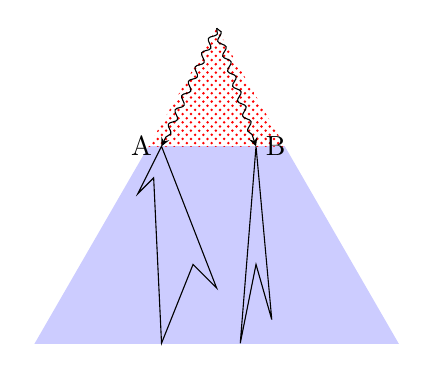
\begin{tikzpicture}
 		
 		
 		
 		\begin{scope}
	 		\clip (-2.4,-1) rectangle (2.4,1.5);
	 		\fill[color=blue!20] (90:3cm) \foreach \x in {210,330} {
	 			-- (\x:3cm)
	 		} -- cycle (60:3cm) ;
 		\end{scope}
 		\begin{scope}
			\clip (-1,1.5) rectangle (1,3);
			\fill[pattern=crosshatch dots, pattern color=red] (90:3cm) \foreach \x in {210,330} {
				-- (\x:3cm)
			} -- cycle (60:3cm) ;
 		\end{scope}
 		\coordinate (nodeA) at (-0.7,1.5);
 		\coordinate (nodeB) at (0.5,1.5);
 		
 		\node at (nodeA) [left] {A};
 		\node at (nodeB) [right] {B};
 		
 		\path[->] (90:3)  edge[snake] (nodeA);
 		\path[->] (90:3)  edge[snake] (nodeB);
 		\draw(nodeA) 
	 			-- (-1,0.9) -- (-0.8,1.1) -- (-0.7,-1) -- (-0.3,0)-- (-0,-0.3) -- cycle;
 		\draw(nodeB) -- (0.3,-1) -- (0.5,0) --  (.7,-0.7) -- cycle;
	\end{tikzpicture}
\end{document}